\documentclass[a4paper, 12pt]{article}
\usepackage[T2A]{fontenc}
\usepackage[utf8]{inputenc} % Важно для корректного отображения кириллицы
\usepackage[english, russian]{babel}
\usepackage{fancyhdr}
\usepackage{indentfirst}
\usepackage{amsmath} % Для математических символов (может пригодиться в отчете)
\usepackage{amsfonts}
\usepackage{graphicx} % Для вставки рисунков (например, логотипа)
\usepackage{tabularx}
\usepackage{geometry}
\usepackage{multicol}
\usepackage{titlesec}
\usepackage{subcaption}
\usepackage{float}
\usepackage{booktabs}
\usepackage{array}   % для улучшенного форматирования таблиц
\usepackage{siunitx} % для выравнивания чисел по десятичной точке
\usepackage[group-digits=false]{siunitx} % ОТКЛЮЧИТЬ разделители тысяч
\usepackage{diagbox}

\titlelabel{\thetitle.\quad}
\geometry{left=2.5cm,right=2.5cm,top=3cm,bottom=2.5cm}
%\geometry{showframe}
\newcommand{\manualtag}[2]{%
    \begingroup
    \renewcommand{\theequation}{#1}% Временная подмена номера
    \refstepcounter{equation}%     % Фиксируем номер для ссылок
    \label{#2}%                    % Ставим метку
    (#1)%                          % Печатаем указанный номер
    \endgroup
}

\begin{document}
\thispagestyle{empty} % Отключаем колонтитулы на этой странице
\begin{titlepage}
	\centering

	{\scshape\large Московский физико-технический институт \par}
    {\scshape (Национальный исследовательский университет) \par}
    
	\vspace{3cm}
	{\LARGE Отчет о выполнении лабораторной работы 1.4.5 \par}
    
	\vspace{1cm}
    {\Huge\bfseries  Изучение колебаний струны \par} 
    
	\vfill
\begin{flushright}
	{\large Выполнил студент группы Б03-501 \\ Середин Николай}
\end{flushright}
	\vspace{2cm}
    г. Долгопрудный
    
    2025
\end{titlepage}

% Настройка колонтитулов для основной части
\pagestyle{fancy} % Включаем продвинутые колонтитулы
\fancyhf{} % Очищаем все установленные по умолчанию колонтитулы
\fancyhead[L]{} % Левый верхний - пустой
\fancyhead[C]{\scshape Лабораторная работа 1.4.5} % Центр верхнего - наш текст
\fancyhead[R]{} % Правый верхний - пустой
%\fancyfoot[C]{\thepage} % Номер страницы по центру вниз
%\fancyfoot[C]{\leaders\hbox to 2pt{\hss-\hss}\hfill\ \thepage\ \leaders\hbox to 2pt{\hss-\hss}\hfill} % Номер страницы по центру в строке с дефисами
\fancyfoot[C]{\rule[0.5ex]{0.05\textwidth}{0.4pt}\quad\thepage\quad\rule[0.5ex]{0.05\textwidth}{0.4pt}}
%\setlength{\parindent}{1.25cm} % Красная строка (абзацный отступ)
\renewcommand{\headrulewidth}{0.4pt}
%\renewcommand{\footrulewidth}{0.4pt}

\newpage
\section{Введение} % Используйте секции для структурирования

{\bfseries Цель работы:} изучить поперечные стоячие волн на тонкой натянутой струне;
измерить собственные частоты колебаний струны и проверить условие образования
стоячих волн; измерить скорость распространения поперечных волн на струне и исследовать её зависимость от натяжения струны.


{\bfseries В работе используются:} закрепленная на станине стальная струна, набор грузов, электромагнитные датчики, звуковой генератор, двухканальный осциллограф,
частотомер.

\section{Теоретические сведения}
\subsection{Волновое уравнение}
Рассмотрим гибкую однородную струну, в которой создано натяжение \(T >>mg\), и получим дифференциальное уравнение, описывающее её малые поперечные свободные колебания. Направим ось \(x\) вдоль струны в положении равновесия. Форму струны будем описывать функцией \(y(x)\), определяющей её вертикальное смещение в точке \(x\) в момент времени \(t\). Угол наклона касательной к струне в точке \(x\) относительно горизонтального направления обозначим как \(\alpha = arctg\frac{\partial y}{\partial x}\).
\begin{figure}[h!]
    \centering
    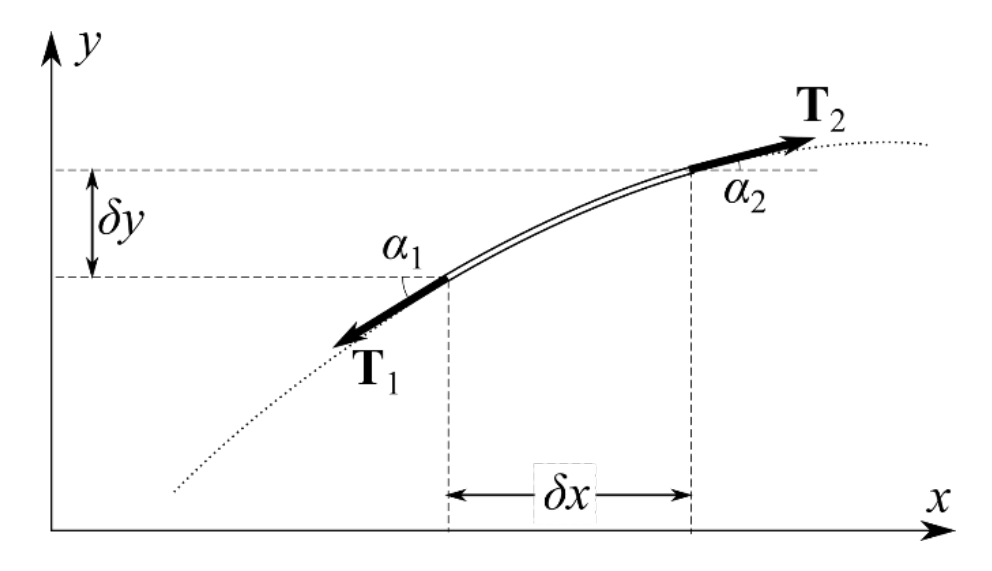
\includegraphics[scale=0.5]{string_equation.png}
    \label{1}
    \caption{К выводу волнового уравнения}
\end{figure}

Второй закон Ньютона для вертикального движения элемента струны запишется в следующем виде:
\[\delta m \ \frac{\partial^2y}{\partial t^2} = -T_1sin\alpha_1 + T_2sin\alpha_2\]
Основываясь на предположении, что отклонения струны от положения равновесия малы, можем сделать ряд упрощений:
\begin{enumerate}
    \item Длина участка струны в смещенном состоянии практически равна длине участка в положении равновесия\footnote{Нетрудно убедиться, что поправка к длине элемента имеет второй (квадратичный) порядок малости по углу \(\alpha\) \(\delta l = \sqrt{\delta y^2 + \delta x^2} = \delta x \sqrt{1+ \frac{\delta y^2}{\delta x^2}} = \delta x \sqrt{1+ tg^2x} \approx \delta x (1+\frac{1}{2}\alpha^2)\)}, поэтому добавочным напряжением вследствие удлинения струны при деформации можно пренебречь. Следовательно, силы \(T_1\) и \(T_2\) по модулю равны силе натяжения струны: \(T_1 \approx T_2 \approx T\).
    \item Углы наклона \(\alpha\) малы, поэтому \(tg \alpha \approx sin \alpha \approx \alpha\), и, следовательно, \(\alpha = \frac{\partial y}{\partial x}\)
\end{enumerate}

\[\rho_l \frac{\partial^2y}{\partial t^2}  = \frac{T_1sin\alpha_1 + T_2sin\alpha_2}{\delta x} \approx T\frac{\alpha_2 - \alpha_2}{\delta x} \rightarrow T\frac{\partial \alpha}{\partial x} = T\frac{\partial (\frac{\partial y}{\partial x})}{\partial x} = T \frac{\partial^2y}{\partial x^2}\]
Получим волновое уравнение, введя величину \(u\) соразмерную скорости.
\[\frac{\partial^2y}{\partial t^2} = u^2 \frac{\partial^2y}{\partial x^2}, \quad \ u = \sqrt{\frac{T}{\rho_l}} \]

\subsection{Бегущие волны}

Покажем, что введённая выше величина \(u\) есть скорость распространения волны на струне. Рассмотрим произвольную функцию вида \(f = f(x - ut)\) Подставляя её в волновое уравнение, убеждаемся, что она является его решением при любом \(f\):
\[\frac{\partial^2 f}{\partial t^2} = \frac{\partial}{\partial x} \left(\frac{\partial f}{\partial \xi}\frac{\partial \xi}{\partial t}\right) = \frac{\partial}{\partial x} \left(-u \frac{\partial f}{\partial \xi}\right) = -u \frac{\partial^2 f}{\partial \xi^2}\frac{\partial \xi}{\partial t} = u^2 \frac{\partial^2 f}{\partial \xi^2}, \ \xi =x-ut \]
\[ \frac{\partial^2 f}{\partial x^2} =  \frac{\partial}{\partial x} \left(\frac{\partial f}{\partial \xi}\frac{\partial \xi}{\partial x}\right) =  \frac{\partial}{\partial x} \left(\frac{\partial f}{\partial \xi} \cdot 1\right) = \frac{\partial^2 f}{\partial \xi^2}\]
\[\frac{\partial^2 f}{\partial t^2} = u^2 \frac{\partial^2 f}{\partial x^2}\]

Как нетрудно видеть, наша функция \(f = f(x - ut)\) описывает возмущение струны произвольной формы, которое смещяется поступательно со скоростью \(u\) вдоль оси \(x\) не меняя своей формы, т.к. \(\xi = const \Rightarrow \frac{\partial \xi}{\partial t} = 0 \Rightarrow \frac{\partial x}{\partial t} = u\).

Как показывается в математических курсах, общее решение дифференциального уравнения в частных производных представимо в виде суммы двух волн произвольной формы, бегущих в противоположные стороны со скоростями \(\pm u\).
\[y(x,t) = y_1(x -ut) + y_2(x+ut)\]
В случае гармонических волн (\(k = \frac{2\pi}{\lambda}\) - волновое число):
\[y(x,t) = acos(\omega t - kx) + bcos(wt+kx), \ u = \frac{\omega}{k} = \nu \lambda\]
Заметим, для малых амплитуд колебаний скорость \(u\) распространения поперечных волн на струне зависит только от силы натяжения струны \(T\) и её погонной
плотности \(\rho_l\), не зависит от модуля Юнга струны (струна считается нерастяжимой) и внешних параметров, таких как амплитуда или частота возбуждающей силы.

\subsection{Собственные колебания струны. Стоячие волны}

Найдем вид свободных колебаний струны с закрепленными концами. Пусть струна закреплена в точках \(x = 0\) и \(x = L\). Концы струны не колеблются, поэтому \(y(0,t) = 0\) и \(y(L,t) = 0\).
\[y(0,t) =  acos(\omega t) + bcos(wt) = 0 \Rightarrow a=-b \Rightarrow y(x,t) = 2asin(kx)sin(\omega t)\]
\(sin(kx) = 0, sin(kx) = 1\) - узлы и пучности соответственно. \(y(L,t)\) - узел, значит, \(sin(kL) = 0 \Rightarrow kL = n\frac{\pi}{2}, \ n \in \mathbb{N}\)
\begin{equation}
    \label{nu_n}
    \nu_n = \frac{u}{\lambda_n} = \frac{n}{2L}\sqrt{\frac{T}{\rho_l}},  \ n \in \mathbb{N}
\end{equation}
\(\nu_n\) - собственные частоты, гармоники струны.

При колебаниях реальной струны всегда имеет место потеря энергии. Для эффективной раскачки колебаний используется явление резонанса — вынуждающая частота должна совпадать с одной из собственных частот струны. Когда потери энергии в точности компенсируются энергией, поступающей от вибратора, колебания струны становятся стационарными и на ней можно наблюдать стоячие волны
\newpage
\section{Экспериментальная установка}

Схема установки приведена на рис. \ref{fig:experimental_setup}. Стальная гитарная струна 1 закрепляется в горизонтальном положении между двумя стойками с зажимами 2 и 3, расположенными на массивной станине 4. Один конец струны закреплен в зажиме 2 неподвижно. К противоположному концу струны, перекинутому через блок, прикреплена платформа с грузами 5, создающими натяжение струны. Зажим 3 можно передвигать по станине, устанавливая требуемую длину струны. Возбуждение и регистрация колебаний струны осуществляются с помощью электромагнитных датчиков (вибраторов), расположенных на станине под струной. Электромагнитный датчик 6 подключен к звуковому генератору 7. Колебания струны регистрируются с помощью электромагнитного датчика 8, сигнал с которого передается на вход осциллографа 9. Разъёмы, через которые датчики с помощью кабелей соединяются с генератором и осциллографом, расположены на корпусе станины.

\begin{figure}[h!]
    \centering
    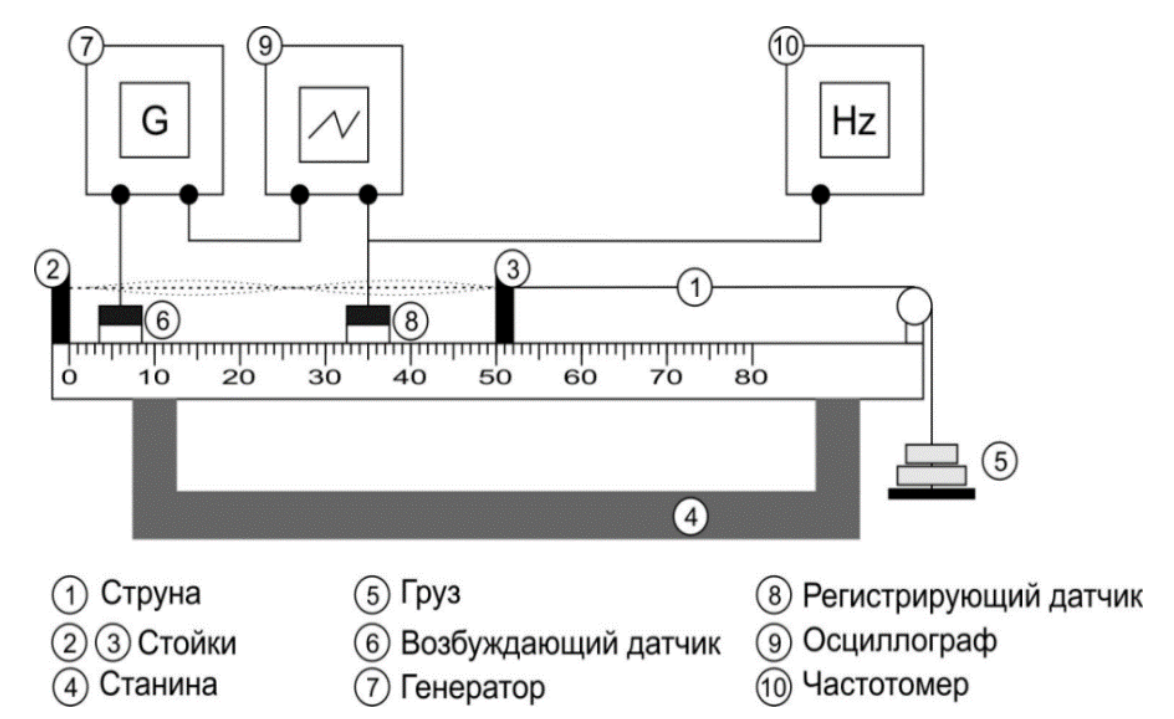
\includegraphics[scale=0.5]{exp_setup.png}
    \caption{Экспериментальная установка}
    \label{fig:experimental_setup}
\end{figure}

Для регистрации колебаний струны в работе используется электронный осциллограф, соединённый с электромагнитным датчиком 8.
\newpage
\section{Ход работы}
\begin{enumerate}
    \item Для разных значений силы натяжения \(T\), т.е с разными массами грузиков, измерим 9 собственных частот струны. Для этого на осциллограф в режиме развертки выведем сигналы генератора и колебаний струны. В момент их относительной остановки и сильного увеличения амлитуды колебаний струны наблюдаем явления резонанса и записываем соответствующее значение собственной частоты. Для большей наглядности расположим датчик приблизительно в пучности (посередине для четных \(\nu_n\), и в \(x_k = \frac{2k-1}{2n}, \ n,k \in \mathbb{N}, \ k\leq n\)). Значение первой гармоники оценим по измеренным заранее погонной плотности \(\rho_l\), и массе грузиков \(m\), используя формулу \ref{nu_n}, где \(T=mg\). Таким образом получим примерные значения \(\nu_n\), далее изменяя частоту генератора ищем положения резонанса возле расчитанных ранее значений.
    \item Построим график \(\nu_n(n)\). По коэффициентам наклона посчитаем \(u(T)\)  и построим график \(u^2(T)\). По коэффициенту наклона найдем \(\rho_l\)
    \[\frac{\nu_n}{n} = \frac{u}{2L}\]
    \[u^2 = \frac{T}{\rho_l}\]
    \item Переключим осциллограф в режим (X-Y) и установим чатоту генератора \(\nu = \nu_1/2\). Получим фигуру Лиссажу. Система имеет высокую гармонику, т.е. теряет небольшое количество энергии и имеет резкий резонанс. Это значит, что кратные субгармоники будут постоянно добавлять одинаковую энергию системе за период, в то время как другие частоты в среднем не будут раскачивать струну. Малые потери энергии и кратные частоты субгармоники раскачивают струну до частоты \(\nu_1\). Очевидно, кратные частоты образуют фигуры Лиссажу на экране осциллографа.
\end{enumerate}

\section{Результаты измерений}

\begin{table}[H]
\centering
\begin{tabular}{|c|c|c|c|c|c|}
\hline
\diagbox{$n$}{$T, \ H$} & 9.76  & 14.61 & 19.44 & 24.35 & 29.2  \\
\hline
1 & 130.1 & 161.2 & 187.7 & 207.2 & 226.4 \\
\hline
2 & 263   & 325   & 377   & 416   & 454   \\
\hline
3 & 395   & 488   & 566   & 625   & 682   \\
\hline
4 & 530   & 651   & 756   & 834   & 910   \\
\hline
5 & 661   & 815   & 945   & 1042  & 1139  \\
\hline
6 & 798   & 979   & 1136  & 1252  & 1367  \\
\hline
7 & 931   & 1144  & 1326  & 1462  & 1596  \\
\hline
8 & 1070  & 1310  & 1518  & 1673  & 1825  \\
\hline
9 & 1195  & 1477  & 1710  & 1884  & 2055  \\
\hline
\end{tabular}
\caption{Зависимость частоты гармоник от \(T\)}
\label{tab:data}
\end{table}

\begin{figure}[H]
    \centering
    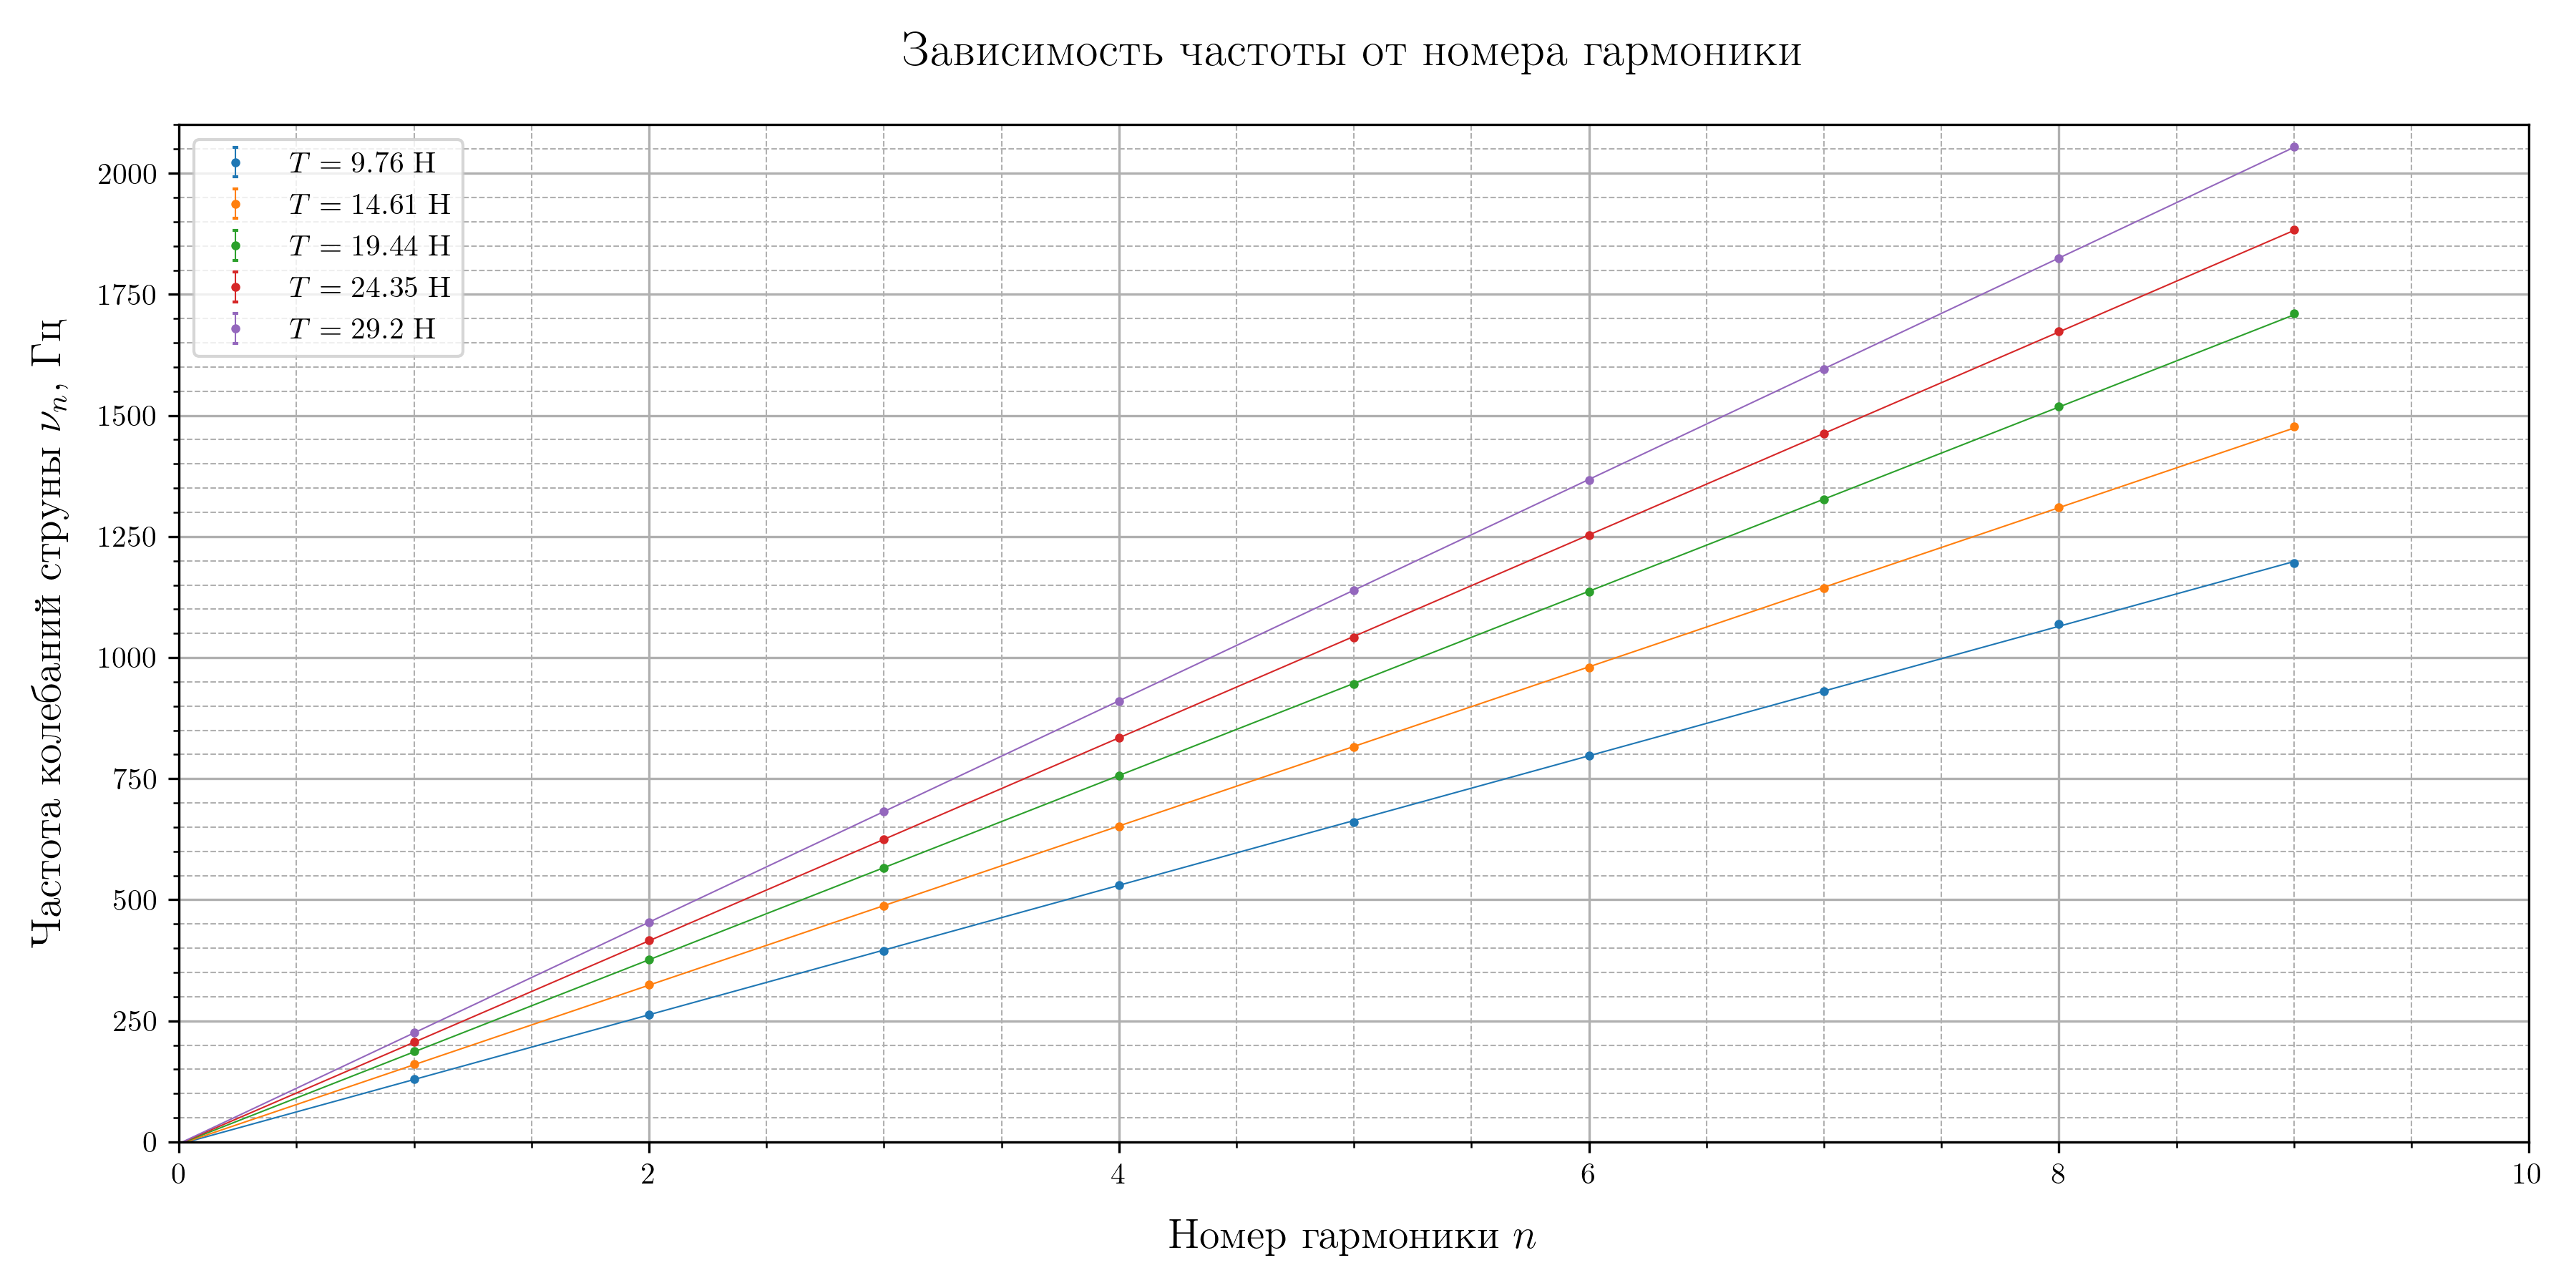
\includegraphics[scale=0.5]{plot.png}
    \label{fig:nu(n)}
\end{figure}
\begin{figure}[h!]
    \centering
    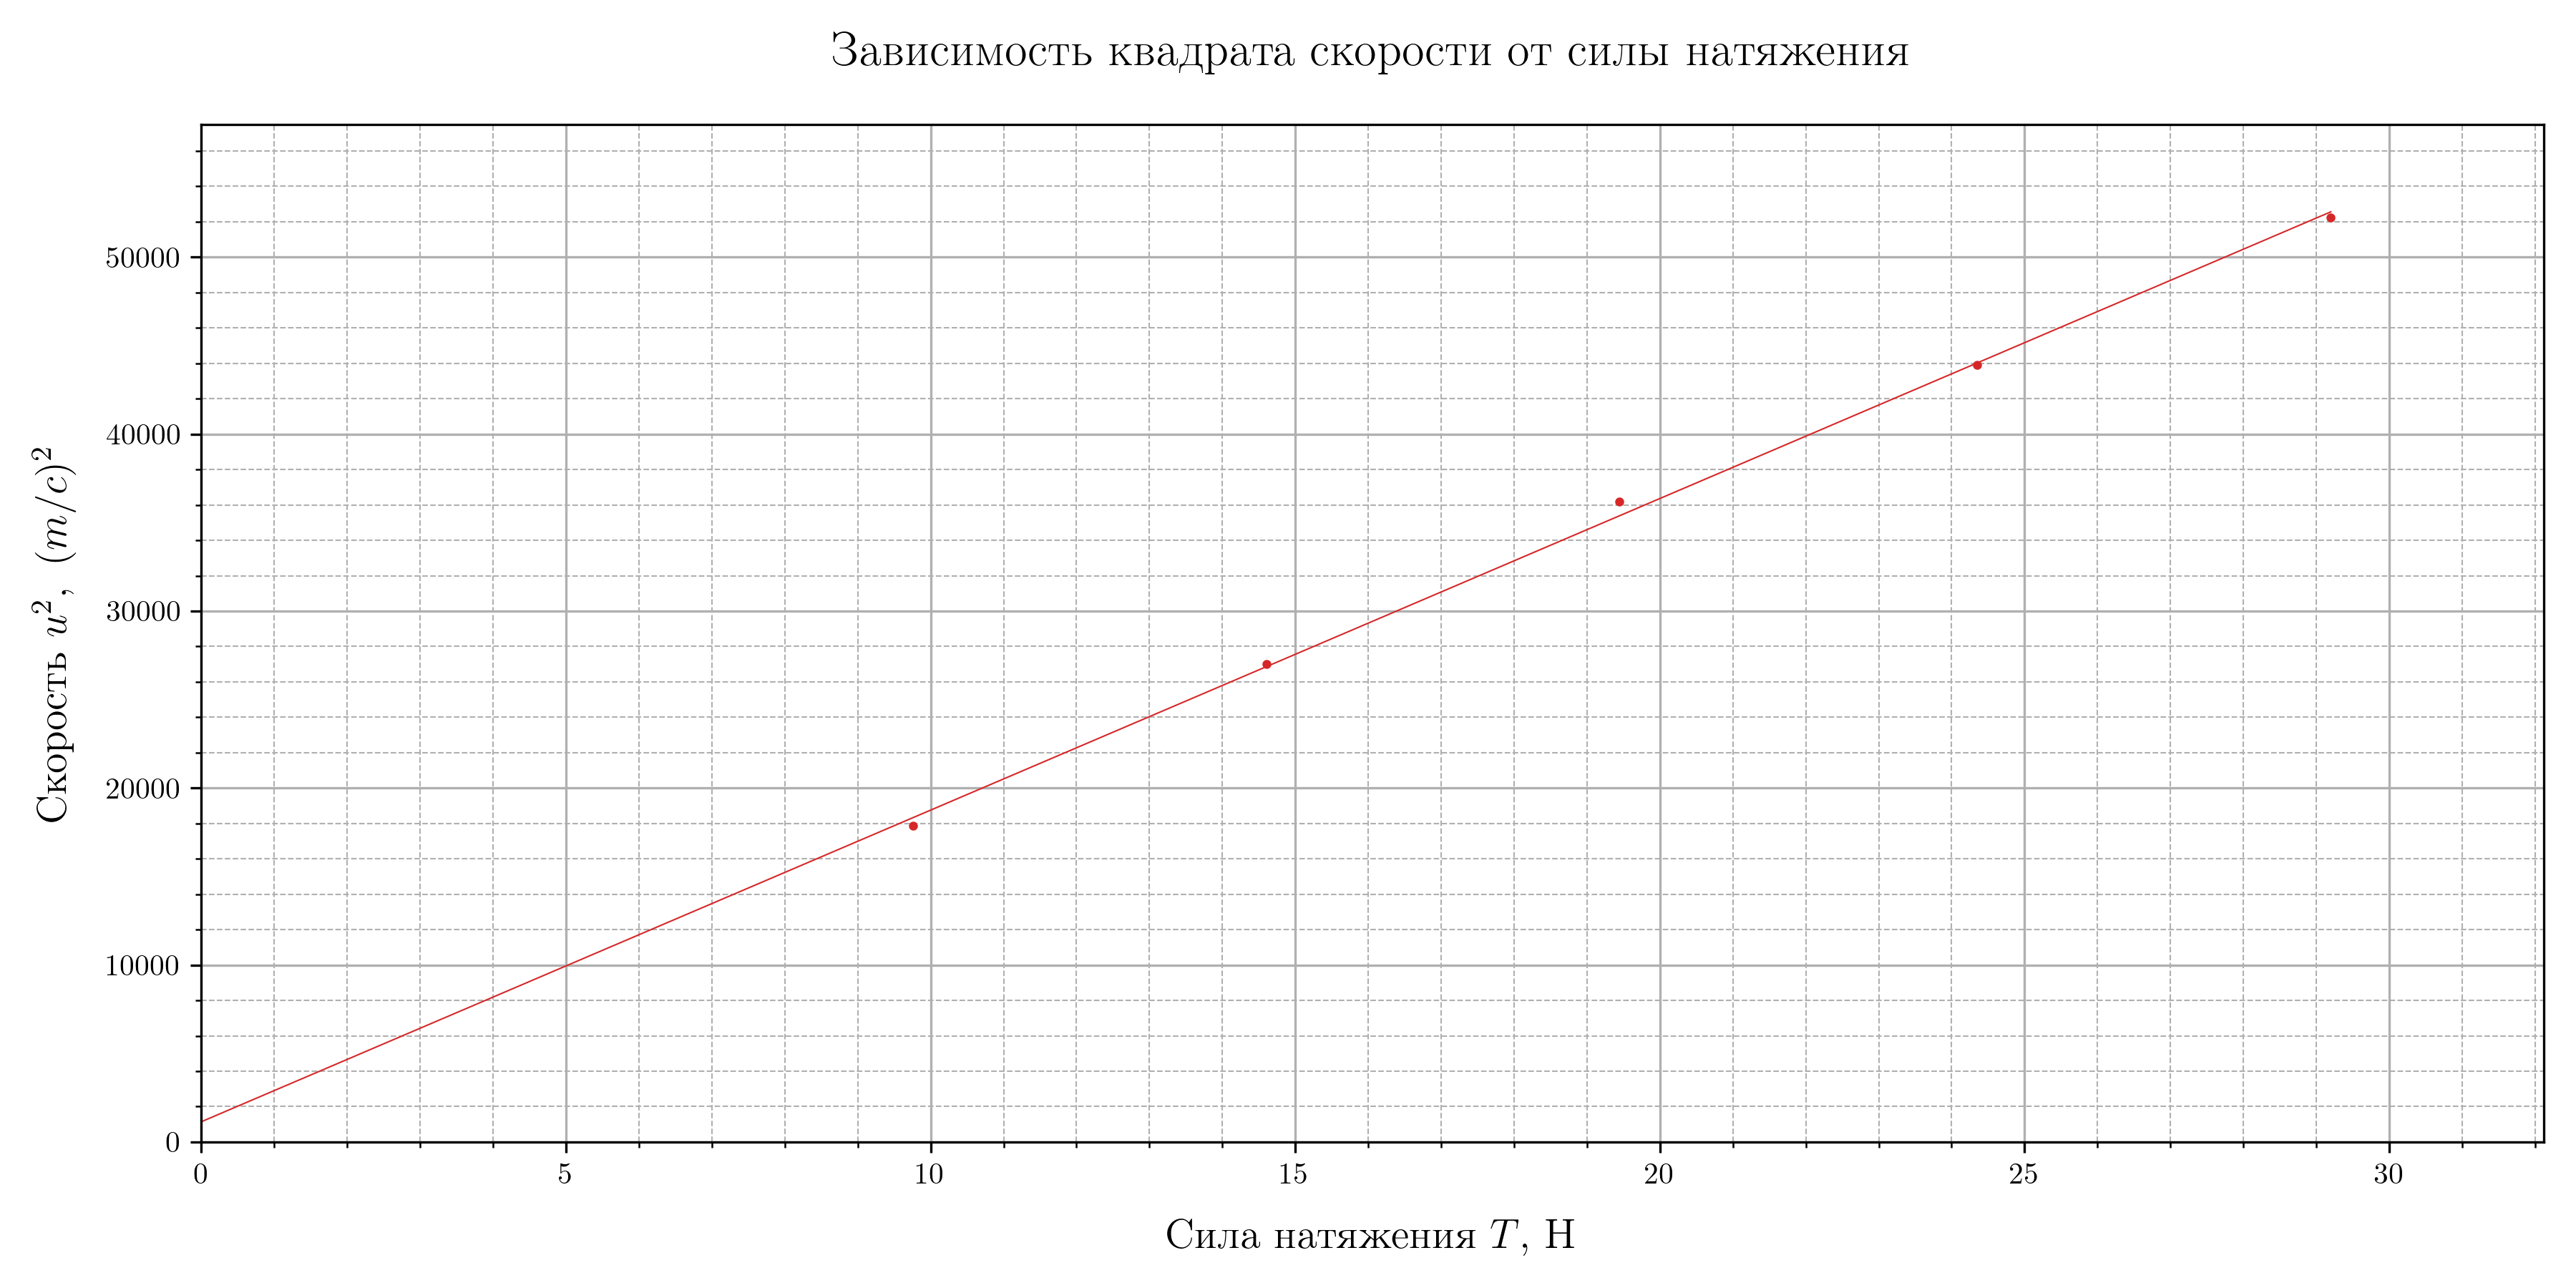
\includegraphics[scale=0.5]{plot2.png}
    \label{fig:u^2(T)}
\end{figure}

\[\textit{Экспериментальные данные} \ \rho_l = (5.68 \ \pm \ 0.10)  \ \cdot \ 10^{-4} \ \textit{кг/м}^3\]
\[ \textit{Параметры установки} \ \rho^{*}_{l} = (5.660 \ \pm \ 0.01)  \ \cdot \ 10^{-4} \ \textit{кг/м}^3\]
\[\varepsilon = \frac{\rho_l - \rho^{*}_{l}}{\rho^{*}_{l}} \approx 0.4 \%\]

\begin{figure}[H]
    \centering
    
    % Первая строка
    \begin{subfigure}[b]{0.45\textwidth}
        \centering
        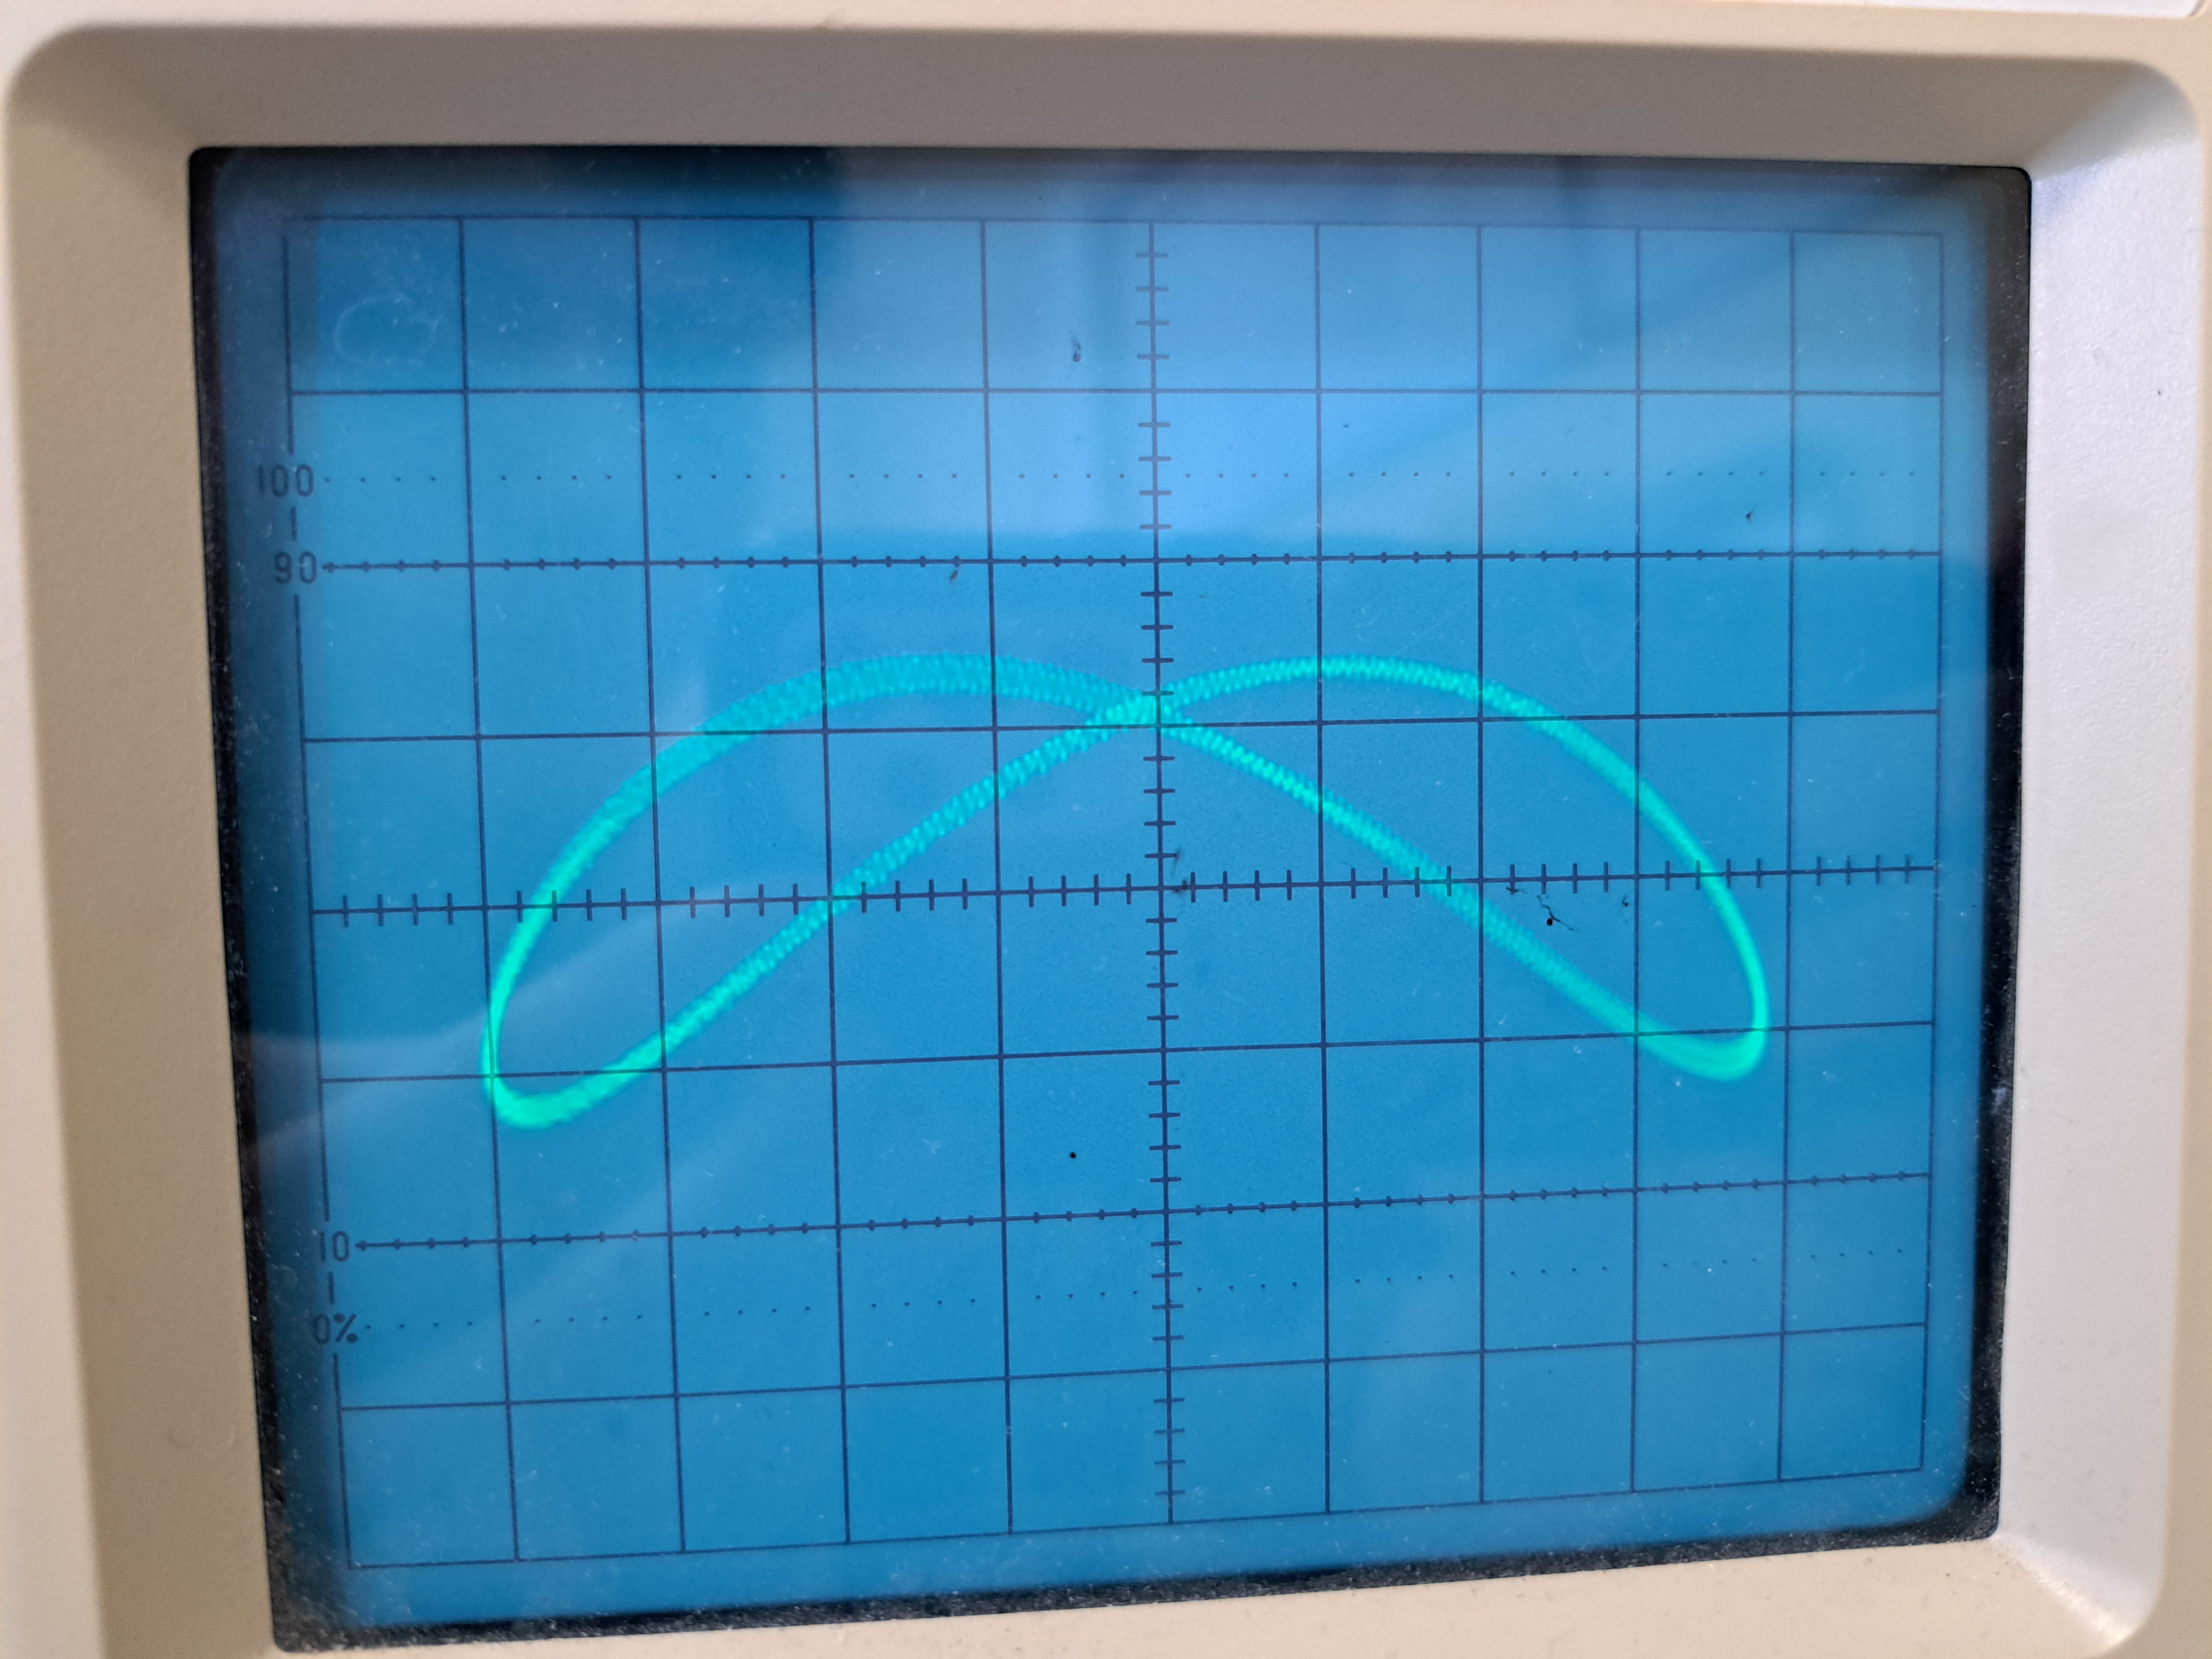
\includegraphics[width=\textwidth]{1.jpg}
    \end{subfigure}
    \hfill
    \begin{subfigure}[b]{0.45\textwidth}
        \centering
        \includegraphics[width=\textwidth]{2.jpg}
    \end{subfigure}
    
    \bigskip 
    
    \begin{subfigure}[b]{0.45\textwidth}
        \centering
        \includegraphics[width=\textwidth]{3.jpg}
    \end{subfigure}
    \hfill
    \begin{subfigure}[b]{0.45\textwidth}
        \centering
        \includegraphics[width=\textwidth]{4.jpg}
    \end{subfigure}
    
    \caption{Фигуры Лиссажу}
    \label{fig:all_four}
\end{figure}



\section{Выводы}
Удалось экспериментально проверить теоретические зависимости и посчитать значение \(\rho_l\), которое с точностью \(0.4\%\) совпадает с посчитанным другим методом. 


\end{document}